\subsection{Controllers for x$_{\mathrm{I}}$ and y$_{\mathrm{I}}$ Directions}
The design of the controllers for the translational movement in $x_{\mathrm{I}}$ and $y_{\mathrm{I}}$ directions is done using the transfer functions of the plant.

The linear equations for the translational model, derived in \autoref{chap:Model}, relate these movements with the roll and the pitch that the quadcopter has at each instant.
%
\begin{flalign}
    m \ddot{x}_{\mathrm{I}} &= -k_{\mathrm{th}} ({\overline{\omega}_1}^2+{\overline{\omega}_2}^2+{\overline{\omega}_3}^2+{\overline{\omega}_4}^2) \theta \label{eq:model_x_transl} \\
    m \ddot{y}_{\mathrm{I}} &=  k_{\mathrm{th}} ({\overline{\omega}_1}^2+{\overline{\omega}_2}^2+{\overline{\omega}_3}^2+{\overline{\omega}_4}^2) \phi \label{eq:model_y_transl} 
\end{flalign} 
Notice that the notation $\Delta$, which correspond to the change from the linearization point, is removed from these equation to avoid excessive notation.

Laplace transforming \autoref{eq:model_x_transl} and \ref{eq:model_y_transl} yields:
%
\begin{flalign}
    m \dot{x}_{\mathrm{I}} s&=-k_{\mathrm{th}}  ({\overline{\omega}_1}^2+{\overline{\omega}_2}^2+{\overline{\omega}_3}^2+{\overline{\omega}_4}^2) \theta \\
    m \dot{y}_{\mathrm{I}} s&= k_{\mathrm{th}} ({\overline{\omega}_1}^2+{\overline{\omega}_2}^2+{\overline{\omega}_3}^2+{\overline{\omega}_4}^2) \phi
\end{flalign}
%
The inner velocity controller design requires a transfer function from each of the angles to each of the translational velocities. This can be written as:
%
\begin{flalign}
    G_{\dot{x}_{\mathrm{I}}}&=\frac{\dot{x}_{\mathrm{I}} }{\theta }=\frac{-k_{\mathrm{th}} ({\overline{\omega}_1}^2+{\overline{\omega}_2}^2+{\overline{\omega}_3}^2+{\overline{\omega}_4}^2)}{m s}=\frac{K_{\dot{x}_{\mathrm{I}}}}{s} \label{eq:Gxdot} \\
    G_{\dot{y}_{\mathrm{I}}}&=\frac{\dot{y}_{\mathrm{I}} }{\phi }=\frac{k_{\mathrm{th}}({\overline{\omega}_1}^2+{\overline{\omega}_2}^2+{\overline{\omega}_3}^2+{\overline{\omega}_4}^2)}{m s}=\frac{K_{\dot{y}_{\mathrm{I}}}}{s}  \label{eq:Gydot}
\end{flalign}
%
\begin{where}
    \va{G_{x_{\mathrm{I}}}}{is the plant for the translational velocity in $x_{\mathrm{I}}$ direction}{m\ s^{-1}\ rad^{-1}}
    \va{G_{y_{\mathrm{I}}}}{is the plant for the translational velocity in $y_{\mathrm{I}}$ direction}{m\ s^{-1}\ rad^{-1}}
\end{where}

From \autoref{eq:Gxdot} and \ref{eq:Gydot} it can be noticed that the two plants are similar but with different sign. The controller design is carried out for the $x_{\mathrm{I}}$ translational velocity and applied to both afterwards, as the design is similar.

The transfer functions are formed by an integrator and a gain. This means the systems are marginally stable in open loop. $G_{x_{\mathrm{I}}}$ has a negative gain, which means that it becomes unstable in closed loop if a controller with positive gain is placed. This feature requires a negative controller gain to compensate for the plant.

It is noticeable that, for this design, the variable changed by the controller is the pitch angle reference for the attitude controller. In order to reduce the effect of the dynamics of the inner loop in the design, the closed loop bandwidth of the outer control loop should be lower.

The bandwidth of the inner attitude control is obtained by making a Bode plot approximation from the pitch angle reference to the real pitch angle in the quadcopter. The obtained Bode diagram is shown in \autoref{fig:bodePitch}. It shows that the bandwidth of the inner loop of 2 rad s$^{-1}$. It has been chosen to set the closed loop bandwidth three times lower than the inner loop. Thus yielding a bandwidth for the velocity control loop of 0.7 rad s$^{-1}$.
%
\begin{figure}[H]
    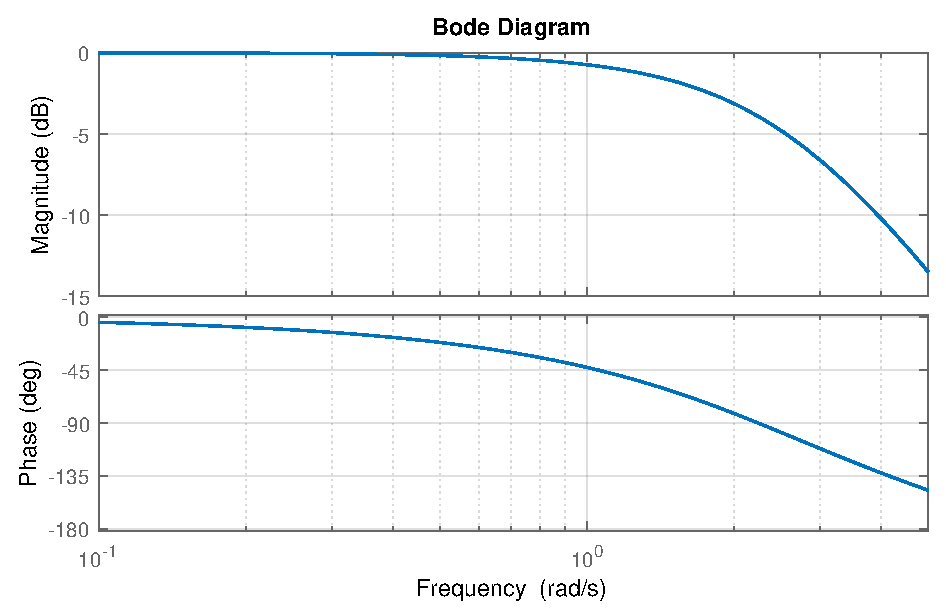
\includegraphics[scale=.7]{figures/bodePitch}
    \centering			
    \captionof{figure}{Attitude control loop Bode diagram.} 
    \label{fig:bodePitch}
\end{figure} 
%
%\begin{flalign}
%        G_{pitch}=\frac{\theta }{\theta_{ref} }=\frac{\omega^2_n}{s^2+\xi  \omega_n  s+\omega^2_n}=\frac{86.05}{s^2+16.14  s+86.05}
%\end{flalign}
%
%With this new dynamics added to the system, the design of the controller can be done. The final rot locus of the plant can be seen in \autoref{fig:rLocusVelocity}.
%%
%\begin{figure}[H]
%    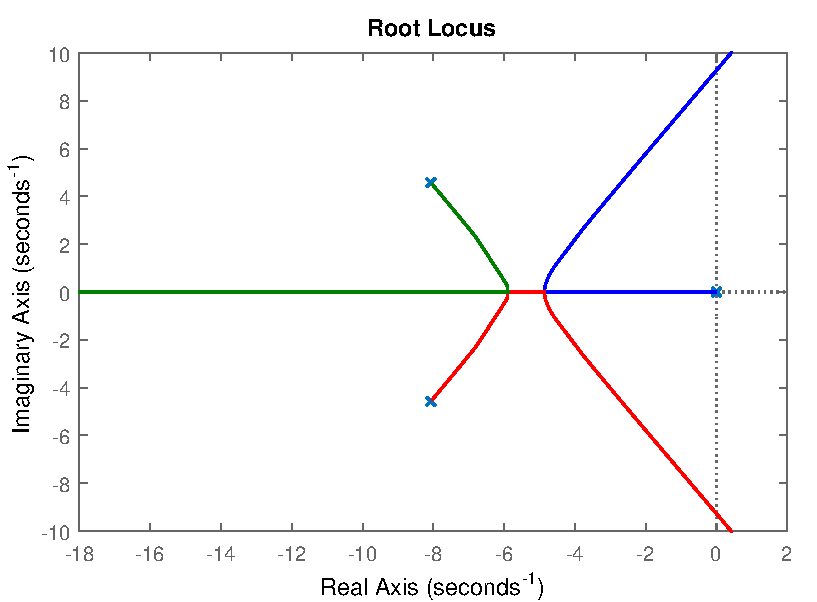
\includegraphics[scale=.7]{figures/rLocusVelocity}
%    \centering			
%    \captionof{figure}{Root locus of the plant for the velocity controller, that includes as well the dynamics of the attitude controller in pitch.} \label{fig:rLocusVelocity}
%\end{figure} 
%
As the plant is a type 1 system, since it contains one integrator, there is no closed loop steady state error if no input disturbances occur. Possible causes for input disturbances are wind, different thrust forces generated in the propellers for the same rotational speed and different rotational speeds in the motors when given the same rotational speed commands.

A diagram of a closed loop system with input disturbance can be seen in \autoref{fig:Feedbackloopswithdisturbance}.
\begin{figure}[H]
    \centering
    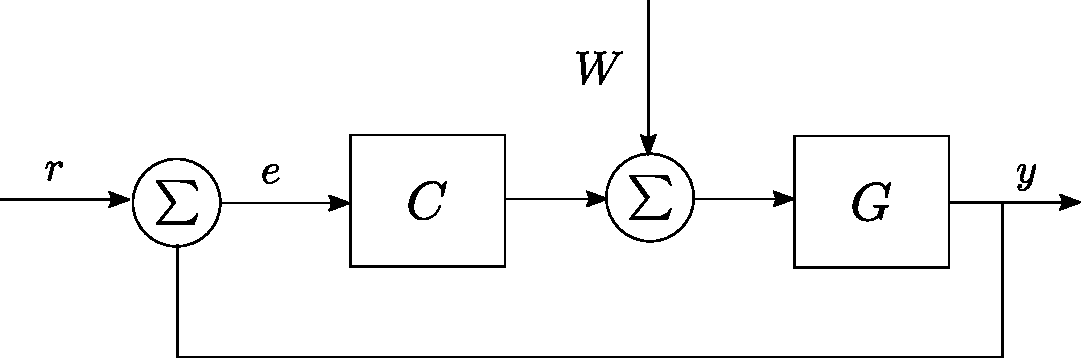
\includegraphics[width=.5\textwidth]{figures/Feedbackloopswithdisturbance.pdf}
    \caption{Feedback loops including input disturbance.}
    \label{fig:Feedbackloopswithdisturbance}
\end{figure}
%
A transfer function for the closed loop from disturbance to output is expressed as
%
\begin{flalign}
    H_{\mathrm{P}}=\frac{G}{1+CG}=\frac{\frac{K}{s}}{1+K_C \frac{K}{s}}=\frac{K}{s+K_C K} \label{eq:dist_tf}
\end{flalign}  
%
The DC gain can be expressed as
\begin{flalign}
 \lim_{s \to 0} H_{\mathrm{P}}=\lim_{s \to 0} \frac{K}{s+K_C K} = \frac{K}{K_C K}\label{eq:dc_gain}
\end{flalign}

As an steady state error is present, an integrator is added to the controller.
\begin{flalign}
H_{\mathrm{PI}}=\frac{G}{1+CG}=\frac{\frac{K}{s}}{1+\frac{K_C}{s} \frac{K}{s}}=\frac{Ks}{s^2+K_C K} \label{eq:dist_tf_integrator}
\end{flalign}  
The DC gain can thereby be given as:
\begin{flalign}
    \lim_{s \to 0} H_{\mathrm{PI}}=\lim_{s \to 0} \frac{Ks}{s^2+K_C K} =0\label{eq:dc_gain_integrator}
\end{flalign}

It is thereby revealed from \autoref{eq:dc_gain_integrator} that the steady state error is eliminated. 

An integrator is therefore included in the control design. Since there already exists an integral term in the plant, the closed loop system becomes marginally unstable since the branches in the root locus are located on the imaginary axis. In order to move them into the left half plane, a zero at $-0.05$ is added to the controller. Then, the gain is adjusted to reduce the oscillations. The zero placement keeps the required bandwidth and enables the possibility of a non oscillating behavior. The final root locus can be seen in \autoref{fig:rl_xdot}.
%
\begin{figure}[H]
	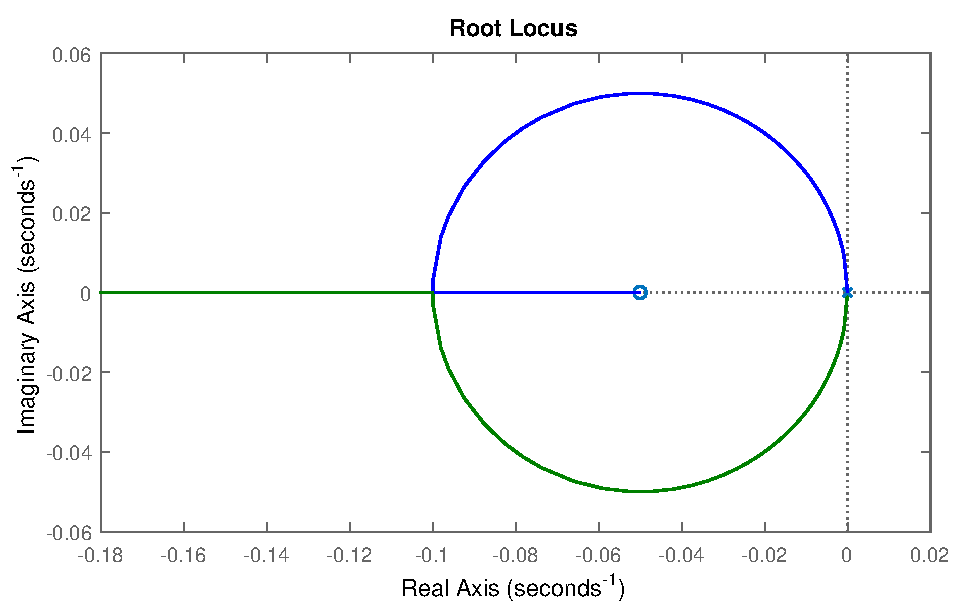
\includegraphics[scale=.7]{figures/rl_xdot}
	\centering			
	\captionof{figure}{Root locus including the plant and the controller for the $x_{\mathrm{I}}$ translational velocity.} 
	\label{fig:rl_xdot}
\end{figure}
%
The Bode plot in \autoref{fig:bodeVelocity} shows that the final bandwidth of the closed loop system is at the desired 0.7 rad s$^-1$.
%
\begin{figure}[H]
	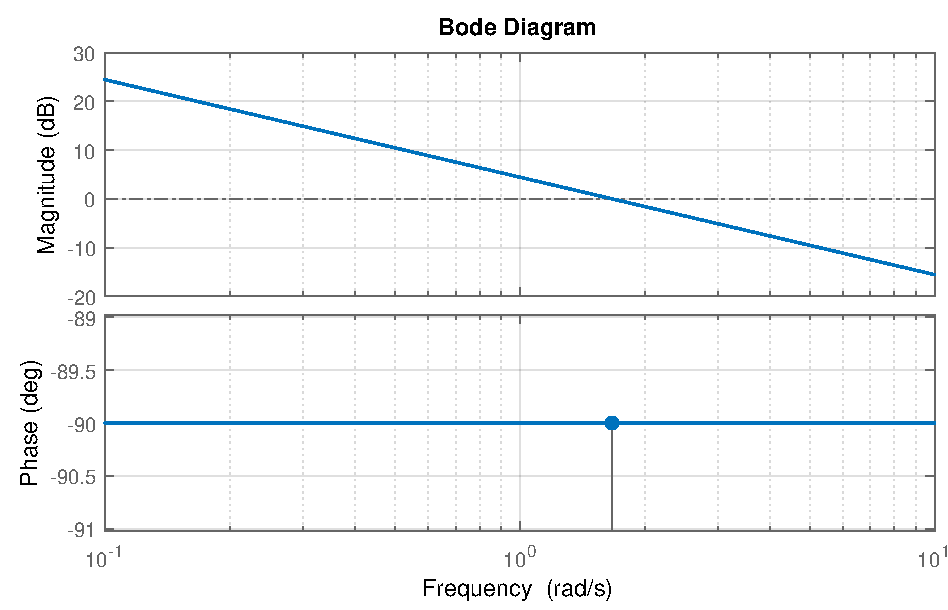
\includegraphics[scale=.7]{figures/bodeVelocity}
	\centering			
	\captionof{figure}{Closed loop Bode of the plant and the controller for the $x_{\mathrm{I}}$ translational velocity.} 
	\label{fig:bodeVelocity}
\end{figure}

The final expression for the controllers for $x_{\mathrm{I}}$ and $x_{\mathrm{I}}$ translational velocity control is written as \autoref{eq:Cxdot} and \ref{eq:Cydot}, respectively. Note, that the plant for the $x_{\mathrm{I}}$ controller has already a positive gain and this makes it unnecessary to include a negative sign in its controller.
%
\begin{flalign}
C_{\dot{x}_{\mathrm{I}}}&= -0.0038\frac{1+20 s}{s} \label{eq:Cxdot} \\
C_{\dot{y}_{\mathrm{I}}}&= 0.0038\frac{1+20 s}{s} \label{eq:Cydot}
\end{flalign}
%
\begin{where}
    \va{C_{\dot{x}_{\mathrm{I}}}}{is the controller for the translational velocity in $x_{\mathrm{I}}$ direction}{rad\ m^{-1}\ s}
    \va{C_{\dot{y}_{\mathrm{I}}}}{is the controller for the translational velocity in $y_{\mathrm{I}}$ direction}{rad\ m^{-1}\ s}
\end{where}

Once the velocity controllers are designed, the position controllers for $x_{\mathrm{I}}$ and $y_{\mathrm{I}}$ directions can be designed by using the same procedure. In this case, the position transfer function is just an integrator as seen in \autoref{eq:Gx} and \ref{eq:Gy}. 
%
\begin{flalign}
G_{x_{\mathrm{I}}}&=\frac{x_{\mathrm{I}} }{\dot{x}_{\mathrm{I}} }=\frac{1}{s}  \label{eq:Gx} \\
G_{y_{\mathrm{I}}}&=\frac{y_{\mathrm{I}} }{\dot{y}_{\mathrm{I}} }=\frac{1}{s}  \label{eq:Gy}
\end{flalign}
%
\begin{where}
    \va{G_{x_{\mathrm{I}}}}{is the plant for the translational position in $x_{\mathrm{I}}$ direction}{m\ s\ m^{-1}}
    \va{G_{y_{\mathrm{I}}}}{is the plant for the translational position in $y_{\mathrm{I}}$ direction}{m\ s\ m^{-1}}
\end{where}

A proportional controller is considered sufficient to control the position of the quadcopter in the x direction as there is an integrator in the plant and the input disturbances are considered in the inner loop.

The proportional gain is chosen so that the bandwidth of the position loop is three times lower than that of the velocity loop. This defines it to be around 0.23 rad s$^-1$. To set this bandwidth, the Bode plot of the plant shown in \autoref{fig:bodePosition} is used. The distance between the gain curve and the 0 dB level at 0.23 rad s$^-1$ sets the gain of the controller to be 0.3.
\begin{figure}[H]
	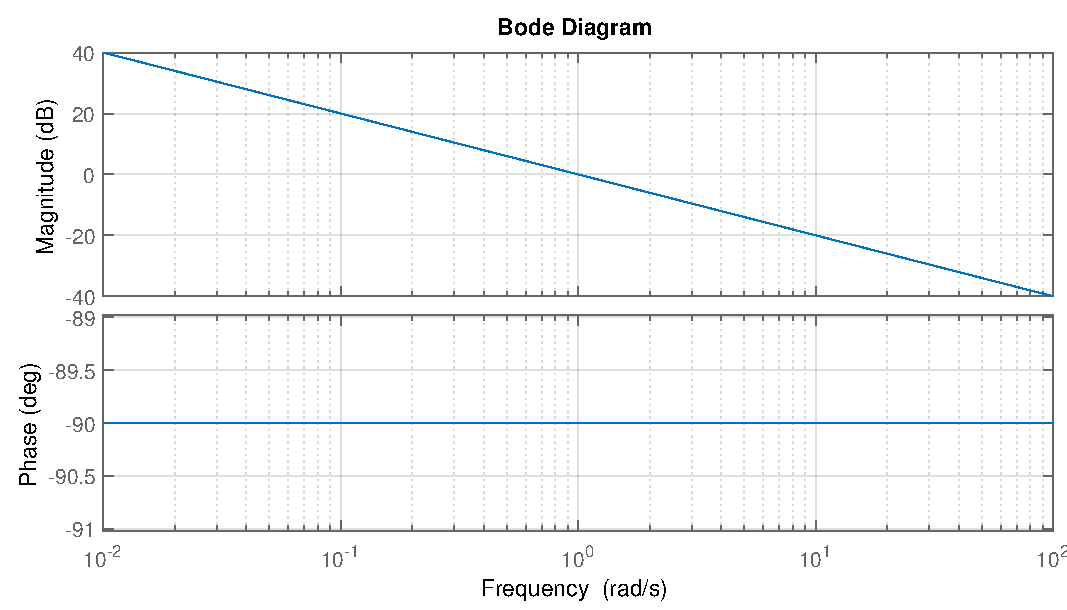
\includegraphics[scale=0.65]{figures/bodePosition}
	\centering			
	\captionof{figure}{Position open loop transfer function Bode diagram for the translational $x_{\mathrm{I}}$ direction.} 
	\label{fig:bodePosition}
\end{figure}
\vspace{-0.8 cm}
The final expression for the translational position controllers can be seen in \autoref{eq:Cx} and \ref{eq:Cy}. In this case, both $x_{\mathrm{I}}$ and $y_{\mathrm{I}}$ controllers are equal.
%
\begin{flalign}
    C_{x_{\mathrm{I}}}&= 0.3 \label{eq:Cx} \\
    C_{y_{\mathrm{I}}}&= 0.3 \label{eq:Cy}
\end{flalign}
%
\begin{where}
    \va{C_{x_{\mathrm{I}}}}{is the controller for the translational position in $x_{\mathrm{I}}$ direction}{m\ s^{-1}\ m^{-1}}
    \va{C_{y_{\mathrm{I}}}}{is the controller for the translational position in $x_{\mathrm{I}}$ direction}{m\ s^{-1}\ m^{-1}}
\end{where}

The translational controllers for the inertial positioning in $x_{\mathrm{I}}$ and $x_{\mathrm{I}}$ have designed. It is thereby possible to simulate the controllers.

%To determine how large the absolute gain can be without making the system unstable due to saturation issues, it is necessary to consider the bandwidth. \ \\
%The data from the Vicon room is transmitted with 100 Hz. This means the attitude controller must run with 50 Hz as maximum to ensure the controller is slower than the sensor data. A rule of thumb states that the bandwidth of the system shall be 25 times smaller than the attitude controller. The desired bandwidth of the translational roll controller is calculated as follows:
%\begin{align}
%BW=2  \pi  \frac{f_s}{25}=2  \pi \frac{50}{25}=12.57\label{eq:bw_X}
%\end{align}
%\begin{where}
%\va{BW}{is the bandwidth of the plant}{rad \cdot s^{-1}}
%\va{f_s}{is the sampling frequency of the plant}{Hz}
%\end{where}
%
%From \autoref{eq:bw_X} it is known, that the ideal bandwidth of the system is 12.57 rad s$^{-1}$. 
%\begin{figure}[H]
%	\centering
%	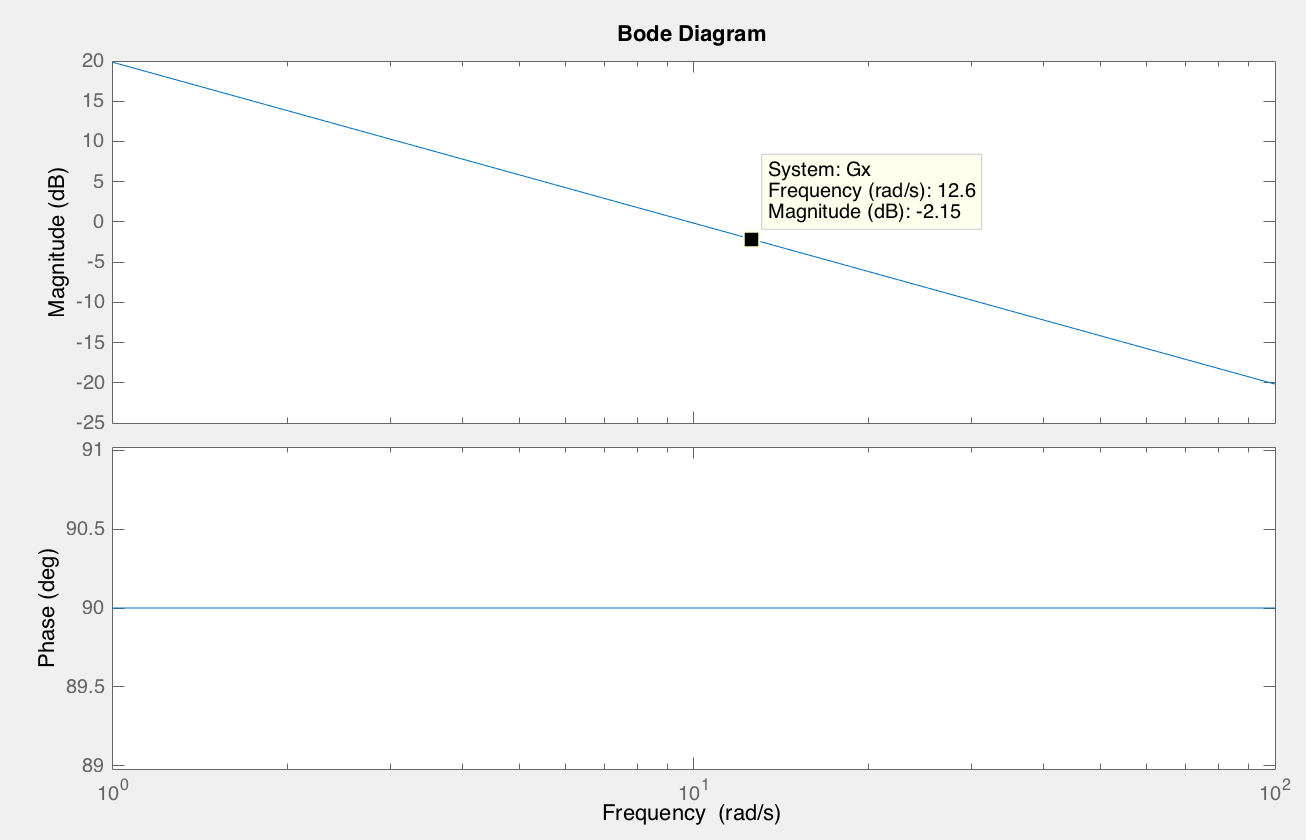
\includegraphics[width=0.7\textwidth]{figures/bode_x.png}
%	\caption{Bodeplot of the plant, with the bandwidth of 12.6 rad s$^{-1}$ displayed.}\label{fig:bode_x}
%\end{figure}
%The bodeplot in \autoref{fig:bode_x} reveals that the magnitude is -2.15 dB at 12.6 rad s$^{-1}$ and must be lowered by 0.85 dB. 

%The gain of the P-controller is found to be: 
%\begin{align}
%C_{x,y}=10^{\frac{-0.85}{20}}=0.907\\
%\end{align}

%The step response for the designed controller can be seen in \autoref{fig:step_x}
%\begin{figure}[H]
%	\centering
%	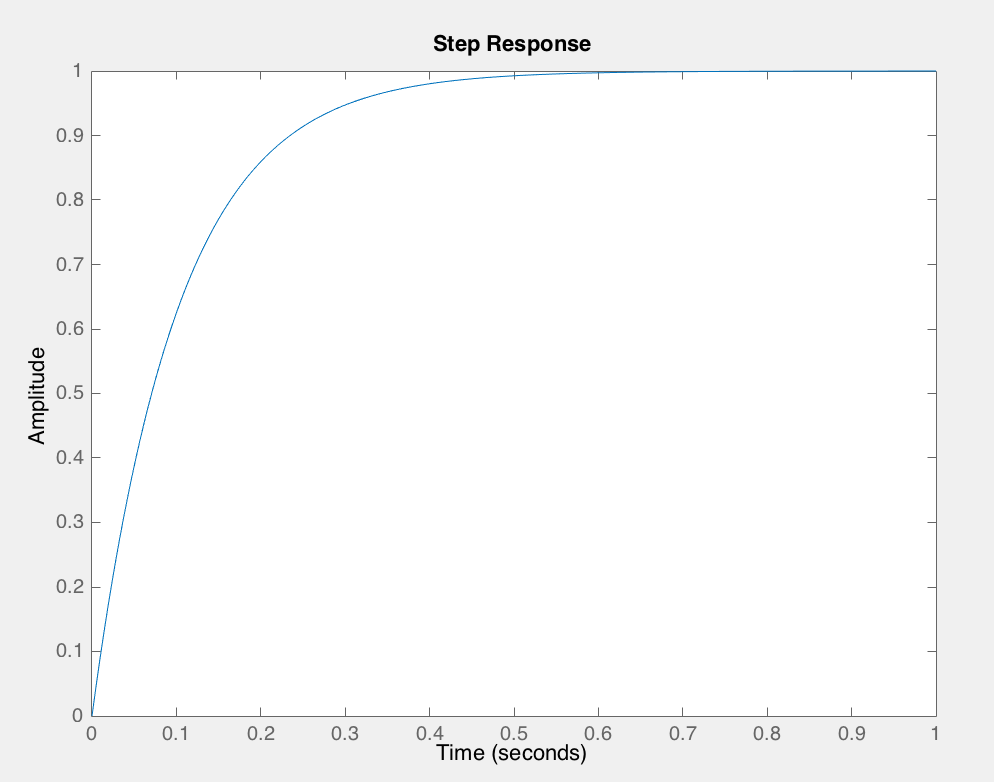
\includegraphics[width=0.8\textwidth]{figures/step_x.png}
%	\caption{Step response for P-controller with a gain of -0.907 and 0.907 for x and y respectively.}\label{fig:step_x}
%\end{figure}
%When examining \autoref{fig:step_x}it is seen that, as expected,there is no steady state error. The system settles at 0.41 seconds and has a rise time of 0.12 seconds. Both settling time and rise time is within the requirements \fxnote{we have not set the requirements - i just wrote it, it seems reasonable, but at some point we must set requirements, that are argued for in a previous chater that is to be written}. As it is a first order system, there is no overshoot and it can therefore be concluded that the P-controller meets all requirements.
%\\
%\\
%Before it can be implemented and tested on the quadcopter, it needs to be discretized. As it is P-controllers, it simply means to encounter the sampling rate. The discretized controllers are presented along with the continuous controller in \fxnote{make graph}.
%\ \\
  
%\subsubsection*{Pitch translational controller}
%The roll and pitch translational models are very similar and will therefore be designed similarly. The design procedure will be the same as for the translational roll controller.\\

% 
%The desired bandwidth is 12,57 rad s$^{-1}$ as derived in \autoref{eq:bw_X}. 
%\begin{figure}[H]
%	\centering
%	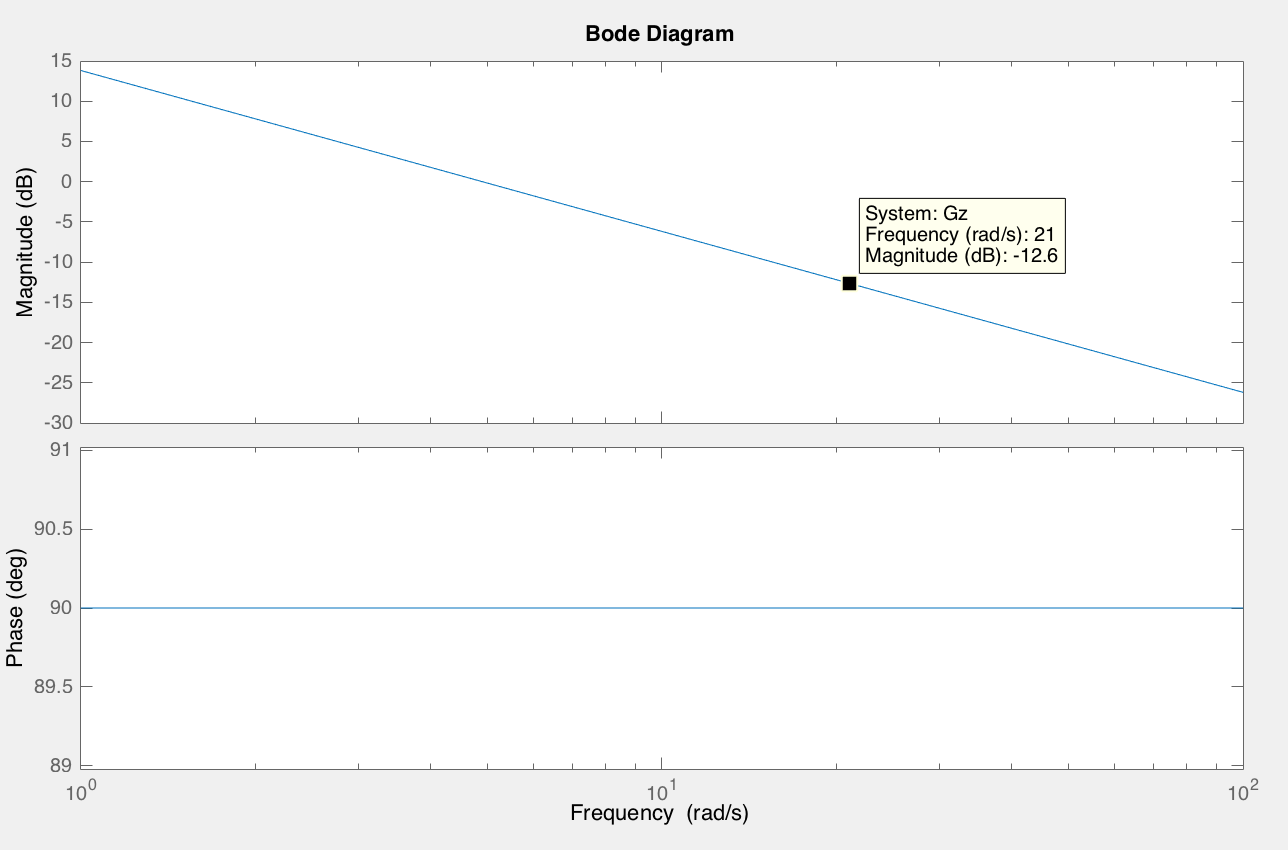
\includegraphics[width=0.7\textwidth]{figures/bode_y.png}
%	\caption{Bode plot of the plant with the 12.6 bandwidth displayed.}\label{fig:bode_y}
%\end{figure}
%The Bode plot in \autoref{fig:bode_z} reveals that the magnitude is -8.2 dB at a magnitude of 12.6 rad s$^{-1}$. The magnitude has to be lifted by 5,2 dB to obtain the desired bandwidth. 




%Before designing the controller limit checks of the transfer function to verify if the model behaves as the plant is expected to in reality is carried out. \\
%\fxfatal{I am having trouble thinking about it, as it is not entirely intuitive to me, when the input is an angle and not a force - however if possible, i think we should have a short piece of text to show we have been critical to the math we have derived - to check it before continuing.} 
%
%Now that the limit checks confirms the sanity of the model, the controller can be designed. \fxnote{I still think that all of the above in this section shall be moved to the model chapter as conclusion of the chapter.}\\
%

%
%FOR NIELS : 
%
%\begin{figure}[H]
%	\centering
%	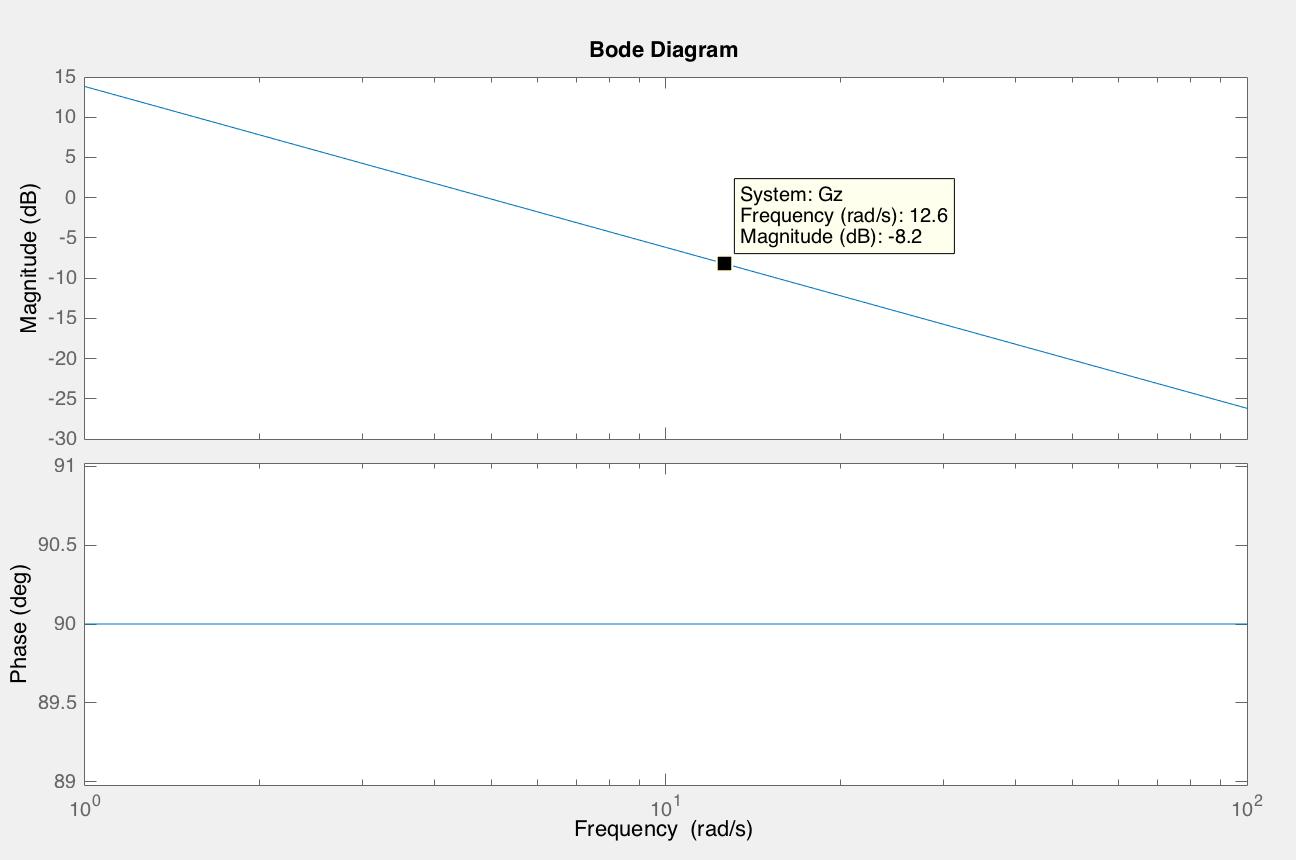
\includegraphics[width=0.7\textwidth]{figures/bode_z.png}
%	\caption{Bode plot of the plant with the 12.6 bandwidth displayed.}\label{fig:bode_z}
%\end{figure}
%The Bode plot in \autoref{fig:bode_z} reveals that the magnitude is -8.2 dB at a magnitude of 12.6 rad s$^{-1}$. The magnitude has to be lifted by 5,2 dB to obtain the desired bandwidth. 
%
%The gain of the P-controller is found to be:
%\begin{align}
%C_y=10^{\frac{5.2}{20}}=1.82
%\end{align}
%The step response can be seen in

%
%The model expression for pitch is previously derived to be:
%\begin{align}
%m\Delta\ddot{y}_{\mathrm{I}} = k_{th}({\overline{\omega}_1}^2+{\overline{\omega}_2}^2+{\overline{\omega}_3}^2+{\overline{\omega}_4}^2)\cos(\overline{\phi})\cos(\overline{\theta})\Delta\phi
%\label{eq:model_y_transl}
%\end{align}
%Laplace transforming \autoref{eq:model_y_transl_y} yields:
%\begin{align}
%m  y_1  s^2= k_{th}  (\omega_1 ^2 + \omega_2 ^2 + \omega_3 ^2 + \omega_4 ^2)  \phi
%\end{align}
%The transfer function for the pitch is as follows:
%\begin{align}
%H_{y1}=\frac{y_1  s}{\phi}=\frac{k_{th}  (\omega_1 ^2 + \omega_2 ^2 + \omega_3 ^2 + \omega_4 ^2)}{m\cdot s}
%\end{align}
%\begin{where}
%\va{H_{y1}}{is the plant for the translational pitch}{1}
%\end{where}
